
\section{Mathematical Background: Category Theory}

The ZX-Calculus is based on the mathematical model of Category-theory. A category is an abstract mathematical model which consists of objects and morphisms. Objects are the building blocks of the category, whereas morphisms act like mappings
between objects. In particular a ZX-diagram is a strict compact
closed symmetric monoidal categor \cite{emmanueljeandel2020zx}.

Given such a category $\mathcal{C}$ with objects $\{A,B,C,D\}$ and morphisms $\{f: A \rightarrow B, g: B \rightarrow C, h: C \rightarrow D\}$, there exists a notion of composition. This means that we can compose morphisms to get new morphisms. In our example, we can compose $f$ and $g$ to get a new morphism $g \circ f: A \rightarrow C$. This composition is associative, meaning that $(h \circ g) \circ f = h \circ (g \circ f)$. Additionally, there exists an identity morphism $id_A: A \rightarrow A$ for each object $A$. This identity morphism is neutral with respect to composition, meaning that $f \circ id_A = f = id_B \circ f$.

There also exists a Bifunctor $\otimes:\mathcal{C}\times\mathcal{C}\rightarrow\mathcal{C}$ which is used to combine multiple \textit{parallel} morphisms into a single morphism. In our example, we can combine $f$ and $g$ to get a new morphism $f \otimes g: A \otimes B \rightarrow C \otimes D$. This Bifunctor is associative, meaning that $(f \otimes g) \otimes h = f \otimes (g \otimes h)$. Additionally, there exists a unit object $I$ which acts as a neutral element with respect to the Bifunctor, meaning that $f \otimes I = f = I \otimes f$ for each morphism $f$.

Furthermore, there exists a natural isomorphism $\sigma_{A,B}: A \otimes B \rightarrow B \otimes A$ for each pair of objects $A$ and $B$. This means that we can always swap the order of parallel morphisms without changing their meaning. This is also called the \textit{swap} rule.


Finally, there also exists a notion of dual objects. Given an object $A$, there exists a dual object $A^*$. Using the special morphisms $\eta_A: I \rightarrow A \otimes A^*$ and $\epsilon_A: A^* \otimes A \rightarrow I$, we can introduce a notion of \textit{curved} morphism. This special morphisms are called \textit{CAP} and \textit{CUP} respectively.

\subsection{Quantum Circuits based on Category Theory}

Using the mathematical model of category theory, we can now define a quantum circuit. For this we are going to restrict our category to the category of finite dimensional Hilbert spaces and linear maps. This means that the objects of our category are finite dimensional Hilbert spaces and the morphisms are linear maps between those Hilbert spaces. We are going to denote this category as $\mathbf{FDHilb}$. Furthermore we define the composition of morphisms as the matrix multiplication of linear maps. The Bifunctor $\otimes$ is defined as the tensor/kronecker product respectively.

We can now define an actual circuit, using this model: For this we are going to look at an entanglement circuit, which creates Bell pairs. This circuit is shown in figure \ref{fig:bell_circuit}. Note that it looks very similar to the normal gate-based circuit. The only difference is that we are translating it in such a way, that we are using the morphisms of our category instead of the gates.

\begin{figure}
    \centering
    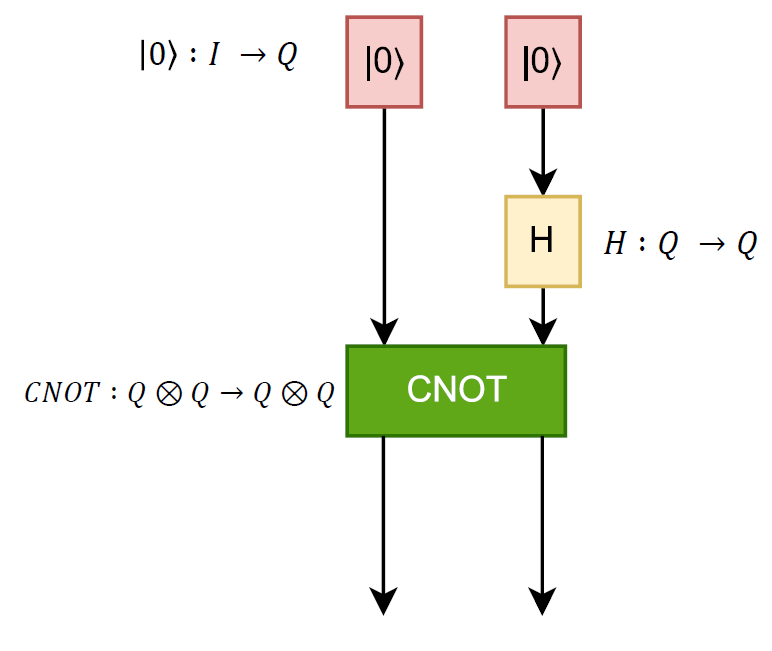
\includegraphics[height=6cm]{images/category-circuit.png}
    \caption{Circuit for creating Bell pairs}
    \label{fig:bell_circuit}
\end{figure}

It uses the following morphisms:

\begin{itemize}
    \item $|0\rangle$ is the morphism $I\rightarrow Q$ which initializes a qubit to the state $|0\rangle$.
    \item $H$ is a morphism of the form $Q\rightarrow Q$. It is a linear map from one qubit to one qubit.
    \item $CNOT$ is the controlled-not gate, which is a linear map from two qubits to two qubits. It is a morphism of the form $Q\otimes Q \rightarrow Q \otimes Q$.
\end{itemize}

At the moment we are only able to define the circuit abstractly. We can not yet define the actual circuit, because we have not yet defined specifically what the objects and morphisms of our category are. We are going to do this in the next section, where we are going to define the Basics of ZX-Calculus.